\documentclass[border=4pt]{standalone}
\usepackage{amsmath}
\usepackage{lmodern}
\usepackage{tikz}
\usetikzlibrary{arrows.meta,calc,positioning,fit,backgrounds}

% 6 pt text: smallest size allowed by the spec (\tiny = 5 pt was too small for IEEE)
\newcommand{\tn}{\fontsize{6pt}{7.2pt}\selectfont}

\definecolor{zonefill}{RGB}{243,245,248}
\definecolor{zoneln}{RGB}{176,185,199}
\definecolor{rtln}{RGB}{196,203,213}
\definecolor{offfill}{RGB}{233,237,242}
\definecolor{offln}{RGB}{148,157,170}
\definecolor{blkln}{RGB}{100,116,139}
\definecolor{planln}{RGB}{55,65,81}
\definecolor{plantfill}{RGB}{233,242,253}
\definecolor{plantln}{RGB}{74,127,193}
\definecolor{accent}{RGB}{42,120,214}
\definecolor{accentdark}{RGB}{23,68,166}
\definecolor{cboxfill}{RGB}{234,242,253}
\definecolor{amfill}{RGB}{253,247,232}
\definecolor{amln}{RGB}{222,170,72}
\definecolor{amtxt}{RGB}{146,104,16}
\definecolor{ink}{RGB}{17,24,39}
\definecolor{graytxt}{RGB}{107,114,128}
\definecolor{fbmid}{RGB}{130,140,150}
\definecolor{fbdark}{RGB}{75,85,99}

\begin{document}
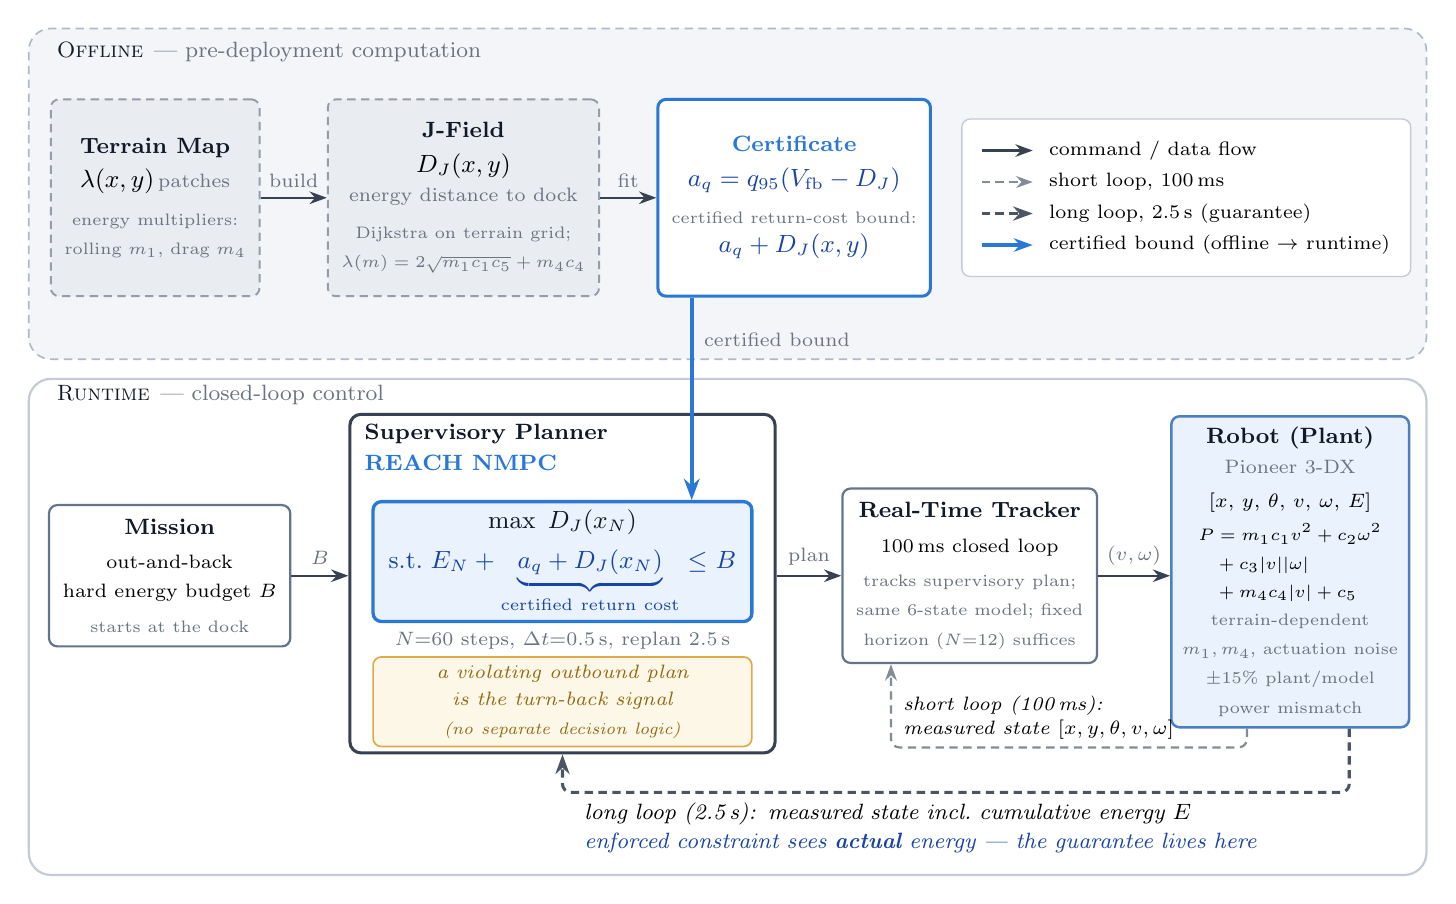
\begin{tikzpicture}[
  font=\footnotesize,
  >={Stealth[length=2.1mm,width=1.5mm]},
  offst/.style={draw=offln,fill=offfill,densely dashed,line width=0.7pt,rounded corners=3pt,align=center,inner sep=5pt},
  certst/.style={draw=accent,fill=white,line width=1.1pt,rounded corners=3pt,align=center,inner sep=5pt},
  rtst/.style={draw=blkln,fill=white,line width=0.8pt,rounded corners=3pt,align=center,inner sep=5pt},
  planst/.style={draw=planln,fill=white,line width=1.1pt,rounded corners=4pt,align=center,inner sep=4pt},
  plantst/.style={draw=plantln,fill=plantfill,line width=0.9pt,rounded corners=3pt,align=center,inner sep=5pt},
  cboxst/.style={draw=accent,fill=cboxfill,line width=1.2pt,rounded corners=3pt,align=center,inner sep=3pt},
  amst/.style={draw=amln,fill=amfill,line width=0.6pt,rounded corners=3pt,align=center,inner sep=3pt},
  legendst/.style={draw=rtln,fill=white,line width=0.5pt,rounded corners=3pt,align=center,inner sep=4pt},
  flow/.style={draw=planln,line width=0.8pt,-{Stealth[length=2.2mm,width=1.6mm]}},
  fbl/.style={draw=fbdark,densely dashed,line width=1.1pt,rounded corners=3pt,-{Stealth[length=2.5mm,width=1.8mm]}},
  fbs/.style={draw=fbmid,densely dashed,line width=0.8pt,rounded corners=3pt,-{Stealth[length=2.1mm,width=1.5mm]}},
  lbl/.style={font=\scriptsize,text=graytxt,inner sep=1.5pt}
]

% ---------------------------------------------------------------- zones
\begin{scope}[on background layer]
  \draw[fill=zonefill,draw=zoneln,densely dashed,line width=0.6pt,rounded corners=8pt]
    (0.1,5.55) rectangle (17.85,9.75);
  \draw[fill=white,draw=rtln,line width=0.8pt,rounded corners=8pt]
    (0.1,-1.00) rectangle (17.85,5.3);
\end{scope}

\node[anchor=south west,inner sep=0pt] at (0.45,9.32)
  {\footnotesize\textsc{\textcolor{ink}{Offline}}\hspace{0.45em}{\footnotesize\color{graytxt}--- pre-deployment computation}};
\node[anchor=south west,inner sep=0pt] at (0.45,4.97)
  {\footnotesize\textsc{\textcolor{ink}{Runtime}}\hspace{0.45em}{\footnotesize\color{graytxt}--- closed-loop control}};

% ---------------------------------------------------------------- OFFLINE
\node[offst,minimum height=2.5cm] (terrain) at (1.705,7.6)
  {{\footnotesize\bfseries\textcolor{ink}{Terrain Map}}\\[3pt]
   {\small$\lambda(x,y)$}\,{\scriptsize\color{graytxt}patches}\\[4pt]
   {\tn\color{graytxt}energy multipliers:}\\[1pt]
   {\tn\color{graytxt}rolling $m_1$, drag $m_4$}};

\node[offst,minimum height=2.5cm] (jfield) at (5.62,7.6)
  {{\footnotesize\bfseries\textcolor{ink}{J-Field}}\\[3pt]
   {\small$D_J(x,y)$}\\[1pt]
   {\scriptsize\color{graytxt}energy distance to dock}\\[4pt]
   {\tn\color{graytxt}Dijkstra on terrain grid;}\\[1pt]
   {\tn\color{graytxt}$\lambda(m) = 2\sqrt{m_1 c_1 c_5} + m_4 c_4$}};

\node[certst,minimum height=2.5cm] (cert) at (9.82,7.6)
  {{\footnotesize\bfseries\textcolor{accent}{Certificate}}\\[3pt]
   {\small\color{accentdark}$a_q = q_{95}(V_{\mathrm{fb}} - D_J)$}\\[4pt]
   {\tn\color{graytxt}certified return-cost bound:}\\[1pt]
   {\small\color{accentdark}$a_q + D_J(x,y)$}};

% legend
\node[legendst,minimum width=5.7cm,minimum height=2.0cm] (legend) at (14.8,7.6) {};
\draw[flow] (12.2,8.2) -- (12.85,8.2);
\node[anchor=west,inner sep=0pt] at (13.05,8.2) {\scriptsize command / data flow};
\draw[fbs] (12.2,7.8) -- (12.85,7.8);
\node[anchor=west,inner sep=0pt] at (13.05,7.8) {\scriptsize short loop, 100\,ms};
\draw[fbl] (12.2,7.4) -- (12.85,7.4);
\node[anchor=west,inner sep=0pt] at (13.05,7.4) {\scriptsize long loop, 2.5\,s (guarantee)};
\draw[accent,line width=1.6pt,-{Stealth[length=2.4mm,width=1.7mm]}] (12.2,7.0) -- (12.85,7.0);
\node[anchor=west,inner sep=0pt] at (13.05,7.0) {\scriptsize certified bound (offline $\to$ runtime)};

% ---------------------------------------------------------------- RUNTIME
\node[rtst,minimum height=1.75cm] (mission) at (1.889,2.8)
  {{\footnotesize\bfseries\textcolor{ink}{Mission}}\\[3pt]
   {\scriptsize out-and-back}\\[1pt]
   {\scriptsize hard energy budget $B$}\\[3pt]
   {\tn\color{graytxt}starts at the dock}};

\node[planst,minimum width=5.4cm,minimum height=4.3cm] (planner) at (6.878,2.7) {};

\node[anchor=north west,inner sep=0pt,align=left] at ($(planner.north west)+(0.2,-0.14)$)
  {{\footnotesize\bfseries\textcolor{ink}{Supervisory Planner}}\\[1.5pt]
   {\footnotesize\bfseries\textcolor{accent}{REACH NMPC}}};

\node[cboxst,text width=4.6cm] (cbox) at (6.878,2.98)
  {{\small\color{ink}$\max\ D_J(x_N)$}\\[5pt]
   {\small\color{accentdark}s.t.\ $E_N + \underbrace{a_q + D_J(x_N)}_{\text{\tn certified return cost}} \le B$}};

\node[inner sep=1pt] at (6.878,1.98)
  {\scriptsize\color{graytxt}$N{=}60$ steps, $\Delta t{=}0.5\,$s, replan $2.5\,$s};

\node[amst,text width=4.6cm] at (6.878,1.2)
  {{\scriptsize\itshape\color{amtxt}a violating outbound plan is the turn-back signal}\\[1pt]
   {\tn\itshape\color{amtxt}(no separate decision logic)}};

\node[rtst,minimum height=2.0cm] (tracker) at (12.05,2.8)
  {{\footnotesize\bfseries\textcolor{ink}{Real-Time Tracker}}\\[3pt]
   {\scriptsize $100\,$ms closed loop}\\[3pt]
   {\tn\color{graytxt}tracks supervisory plan;}\\[1pt]
   {\tn\color{graytxt}same 6-state model; fixed}\\[1pt]
   {\tn\color{graytxt}horizon ($N{=}12$) suffices}};

\node[plantst,inner sep=4pt] (robot) at (16.12,2.85)
  {{\footnotesize\bfseries\textcolor{ink}{Robot (Plant)}}\\[1pt]
   {\scriptsize\color{graytxt}Pioneer 3-DX}\\[3pt]
   {\scriptsize $[x,\, y,\, \theta,\, v,\, \omega,\, E]$}\\[3pt]
   {\tn $\begin{aligned}P &= m_1 c_1 v^2 + c_2 \omega^2\\
        &{}+ c_3|v||\omega|\\
        &{}+ m_4 c_4|v| + c_5\end{aligned}$}\\[3pt]
   {\tn\color{graytxt}terrain-dependent}\\[1pt]
   {\tn\color{graytxt}$m_1, m_4$, actuation noise}\\[1pt]
   {\tn\color{graytxt}$\pm 15\%$ plant/model}\\[1pt]
   {\tn\color{graytxt}power mismatch}};

% ---------------------------------------------------------------- main flow
\draw[flow] (mission.east |- 0,2.8) -- (planner.west |- 0,2.8)
  node[midway,above=2pt,lbl] {$B$};
\draw[flow] (planner.east |- 0,2.8) -- (tracker.west |- 0,2.8)
  node[midway,above=2pt,lbl] {plan};
\draw[flow] (tracker.east |- 0,2.8) -- (robot.west |- 0,2.8)
  node[midway,above=2pt,lbl] {$(v,\omega)$};
\draw[flow] (terrain) -- (jfield) node[midway,above=2pt,lbl] {build};
\draw[flow] (jfield) -- (cert) node[midway,above=2pt,lbl] {fit};

% ---------------------------------------------------------------- certified bound (emphasised)
% Drops from the Certificate straight onto the constraint box, clear of its corner
% and of the planner title.
\coordinate (dropx) at ($(cert.south west)+(0.45,0)$);
\draw[accent,line width=1.6pt,-{Stealth[length=2.7mm,width=2mm]}]
  (dropx) -- (cbox.north -| dropx);
\node[anchor=south west,inner sep=0pt] at ($(dropx)+(0.15,-0.62)$)
  {\scriptsize\color{graytxt}certified bound};

% ---------------------------------------------------------------- feedback loops
% Both routes are strictly orthogonal and never cross.
%   short (inner, light)  : robot -> tracker, 100 ms
%   long  (outer, heavy)  : robot -> planner, 2.5 s, carries E
\coordinate (shortX) at ($(robot.south)+(-0.55,0)$);
\coordinate (longX)  at ($(robot.south)+(0.75,0)$);

\draw[fbs]
  (shortX) -- (shortX |- 0,0.62)
           -- (11.05,0.62)
           -- (tracker.south -| 11.05,0);

\draw[fbl]
  (longX) -- (longX |- 0,0.05)
          -- (6.878,0.05)
          -- (planner.south);

\node[anchor=south west,inner sep=0pt,align=left]
  at (11.2,0.72)
  {\scriptsize\itshape short loop (100\,ms):\\[-1pt]
   \scriptsize\itshape measured state $[x,y,\theta,v,\omega]$};

\node[anchor=north west,inner sep=0pt,align=left,text width=10.4cm]
  at (7.15,-0.08)
  {\footnotesize\itshape long loop (2.5\,s): measured state incl.\ cumulative energy $E$\\[1pt]
   \footnotesize\itshape\textcolor{accentdark}{enforced constraint sees \textbf{actual} energy --- the guarantee lives here}};

\end{tikzpicture}
\end{document}